\documentclass[12pt, oneside, a4paper, bibgerm, numbers=noenddot, parskip=half]{scrreprt}
\usepackage[T1]{fontenc} 

\headheight 50pt

\setcounter{secnumdepth}{3}
\setcounter{tocdepth}{3}

\usepackage[german, english]{babel}
\usepackage[utf8]{inputenc}
\usepackage[T1]{fontenc}

\usepackage{graphicx}
\usepackage{placeins}
\usepackage{subfig}
\usepackage{bibgerm}
\usepackage{url}
\bibliographystyle{alphadin}

\usepackage{algorithm}
\usepackage{algpseudocode}
\algrenewcommand\algorithmicrequire{\textbf{Input:}}
\algrenewcommand\algorithmicensure{\textbf{Output:}}

\renewcommand{\familydefault}{\sfdefault}
\renewcommand{\baselinestretch}{1.0}

\makeatletter
\renewcommand\l@figure{\@dottedtocline{1}{0em}{2.6em}}
\renewcommand\l@table{\@dottedtocline{1}{0em}{2.6em}}
\makeatother


\def\mydotfill{
\leaders\hbox to 0.80em{.\hss}\hfill}
\usepackage{nomencl}
\let\abk\nomenclature
\renewcommand{\nomname}{AbkŸrzungsverzeichnis}
\renewcommand{\nompreamble}{\vspace*{0.6\baselineskip}\markboth{\nomname}{\nomname}}
\setlength{\nomlabelwidth}{0.4\textwidth}				% Setzt den Abstand zwischen AbkŸrzung und ErklŠrung
\renewcommand{\nomlabel}[1]{#1 \mydotfill}			% Punkte zwischen AbkŸrzung und ErklŠrung
\setlength{\nomitemsep}{-\parsep}					% ZeilenabstŠnde zwischen den AbkŸrzungen verkleinern
\usepackage[normalem]{ulem}
\newcommand{\markup}[1]{\uline{#1}}
\makenomenclature

\setlength{\parindent}{0pt}

\usepackage{listings}
\usepackage{color}

\definecolor{R.red}{RGB}{187,0,0}
\definecolor{R.green}{RGB}{127,166,0}

\lstset{language=Perl,
	 basicstyle=\small,
	 numbers=left,
	 numberstyle=\small,
	 numbersep=5pt,
	 captionpos=b,
	 keywordstyle=\color{R.red},
	 commentstyle=\color{R.green}
}

\renewcommand{\labelitemi}{--}

\usepackage[percent]{overpic}
\pdfminorversion=5
\usepackage[absolute]{textpos}

\usepackage{ntheorem} 
\usepackage{mathtools} 


\usepackage{float}
\restylefloat{figure}

\usepackage{booktabs}
\usepackage{tabularx}
\usepackage{supertabular}
\usepackage{multirow}
\usepackage{multicol}

\pagestyle{headings}

\lstdefinelanguage{Lua}{%
morekeywords={%
and,break,do,else,elseif,end,false,for,function,if,in,%
local,nil,not,or,repeat,return,then,true,until,while%
},%
sensitive=true,%
morecomment=[l]{--},%
morecomment=[n]{--[[}{]]},%
morestring=[b]",%
morestring=[b]',%
}[keywords,comments,strings]% 

\newcommand{\tc}[1]{\ensuremath{\underline{\smash{\mathit{#1}}}}}

\DeclareMathOperator{\atan2}{atan2}


\begin{document}
\begin{titlepage}


\includegraphics[angle=0,width=10cm]{Titelseite/oth.png}

\begin{center}
\vspace*{2\baselineskip}
\LARGE \textbf{\textsf{\textit{
Evaluation of different methods for Twitter Sentiment Analysis
}}} \\
\vspace{1cm}
\LARGE\textbf{\textsf{\textit{Bachelor's thesis}}} \\
\vspace{1cm}
\Large{
submitted on June 15, 2022 \\
to Prof. Dr. Florian Heinz \\
Faculty for Mathematics und Computer Science \\
Department Databases \\
Ostbayerische Technische Hochschule Regensburg \\
\vspace{1cm}
by \\
Matteo Enrico Hoffmann \\
<matteo.hoffmann@st.oth-regensburg.de> \\
Matriculation number: 3173721 \\
}
\vspace{1cm}

\end{center}

\end{titlepage}





\chapter*{Abstract}
\selectlanguage{german}{Zusammenfassung der Bachelor-Arbeit auf Deutsch und Englisch. (Abstract)}

\selectlanguage{english}
Questions:
\begin{itemize}
\item How much explanation of the methods? --> nicht so viel, so wie ich es gemacht habe
\item Should extraction of tweets be part of the abstract?
\item Should the results be part of the abstract? --> rauslassen, eher Motivation --> contributions Werbung nicht Kurzzusammenfassung,Ziele
\item Motivation/introduction?
Ziele: Was genau soll ermittelt werden, was machen mit diesen Ergebnissen --> results can be used to implement means of evaluating --> Praxisbezug, ein Satz reicht
\end{itemize}


The increasing popularity of social media provides new data sources to determine the public's opinion using sentiment analysis. The aim of this thesis is the evaluation and comparison of three different approaches to this topic.

The first approach is lexicon-based, which determines the overall sentiment by assessing each word using the scores defined by the dictionary. The second method employs a supervised machine learning classifier that is trained on labelled tweets. The last approach combines the previous two in order to overcome some of their drawbacks, such as the intrinsic limitation of using a finite lexicon or the need to provide tweets for training. Each method is executed and then evaluated based on a defined set of parameters using a case study on <insert topic>.

The results show that ...





\tableofcontents		% Fügt das Inhaltsverzeichnis ein
\addtocontents{toc}{\protect\enlargethispage{0.5cm}}


% \pagenumbering{arabic}	% Verwendet als Seitenzahl arabische Ziffern

\chapter{Introduction}
\label{cha:Chapter1_Introduction}

\iffalse

Total length: up to 5 Months = ~20 weeks oder
\selectlanguage{german}{

Abstract fertig machen, konkreter werden --> vor allem Methoden, kleiner Ansatz


Length: 1-2 pages
Inhaltsverzeichnis --> auch mehr Punkte

Methodology and Implementation --> kann man auch anders aufteilen
Motivation, Hintergrund

Warum diese Plattform --> einfache API

Auch aufpassen illegal

Wann schreiben? --> am Anfang, am Ende? Erstmal Entwurf am Ende
}
\selectlanguage{english}
%
%Effort: 1-2 days
%\begin{itemize}
%\item Major importance of social media, impact on politics, source of information
%\item Massive number of posts allows for a good basis for analysis
%\item Analyse current trends, public's opinion on certain issues, news and other topics
%\item Motivation: Condense massive amount of information/opinions into an intelligible format
%\item Chosen platform: Twitter, short messages <280 characters, massive user base, broad topic range
%\end{itemize}
%

\fi
Kaplan and Haenlein define Social Media as "a group of Internet-based applications that build on the ideological and technological foundations of Web 2.0, and that allow the creation and exchange of User Generated Content" \cite[p.~61]{KAPLAN201059}. 

According to Pew Research Center, around 72\% of Americans use any kind of social media, with the most popular platforms being Facebook at 69\%, followed by Instagram at 40\% and Pinterest at 31\%. Different age groups also choose different platforms, as Snapchat is used by over half of 18-29 year olds, while only being used by 2\% of 65+ year olds. Twitter and Facebook on the other hand are the two platforms with the lowest difference between the youngest and oldest usage shares. Most platforms are also often used daily by their users, showing the importance in their daily lives \cite{pew:socialmedia}. Because of these usage numbers, massive amounts of data are created every day, which can and should be utilized through Social Media Mining. Gundecha and Liu identified some key challenges. Community Analysis deals with the detection of communities, Sentiment Analysis deals with the extraction of opinions out of content. Social Recommendation tries to recommend items based on the user's history and other users. Influence Modeling tries to discern whether a community is driven by influence (certain key influencers) or homophily (similarity). Information Diffusion and Provenance wants to analyze how information spreads in social media. Lastly, Privacy, Security, and Trust are very important as Social Media becomes more and more involved in personal life \cite{Gundecha2012MiningSM}.

The number of possible research topics provided by Social Media is enormous. Sentiment Analysis in particular is very interesting due to the inherent human interest in other people's opinions and viewpoints. Social Media allows us to read and discuss opinions with a vast amount of people. Pang and Lee identified several applications for Sentiment Analysis. Reviews are very important to users, and automatic aggregation can be very valuable. Sentiment Analysis also be used as a sub-component, for example in a recommendation system. In addition, business and government intelligence can benefit from sentiment analysis, for example, in reputation management and public relations, but also in product research \cite{pang-etal-2002-thumbs}. In politics especially, the analysis of population attitudes is very important, and Sentiment Analysis could be a supplement to existing polling methods, as shown by Brendan et al. \cite{polls}. 
\TODO{twitter!!}
Thus, it is clear that Sentiment Analysis is a key part of processing Social Media data with a wide variety of applications. Most of the research for Sentiment Analysis can be classified into three main branches. The lexicon-based methods utilize sentiment lexicons which contain sentiment-bearing with their polarity or polarity score. Machine-Learning methods employ machine-learning classifiers, while hybrid methods combine the previous two approaches. Approaches also often utilize different data sets to evaluate their methods, due to a lack of benchmark data sets and the difficulty of annotating Twitter data \cite{DBLP:journals/csur/GiachanouC16}.

The aim of this thesis is the implementation and evaluation of all three approaches using existing data sets. Most research focuses only on one or two approaches and often uses a new data set, which makes comparisons of different approaches more difficult. Thus, this thesis allows for easier categorization both inbetween methods and other research.




\TODO{What does the reader already know --> duplicate info/adapt}




\chapter{Related work}
\label{cha:Chapter2_RelatedWork}
\iffalse

Length: 1-2 pages

Effort: ~2 weeks

2-3 Arbeiten maximal, die genauer betrachtet werden
Ruhig mehr Zitate --> aber nicht detailliert betrachten
Introduction to Data Mining --> zu generell, nur als Zitat
Hier nur im engsten Sinne


Content
\begin{itemize}
\item Alec Go, Richa Bhayani, and Lei Huang. 2009. Twitter Sentiment Classification Using Distant Supervision.
Technical Report. Standford.
\item Taboada or Serendio or Vader?
\item Khuc et al.
\end{itemize}

\fi

Although a large number of Sentiment Analysis focuses on domains such as movie or product reviews, the work considered here concentrates on Twitter Sentiment Analysis. The current state of research is often divided into three different major classes: Machine Learning, Lexicon-Based, and Hybrid. \cite{DBLP:journals/csur/GiachanouC16}. Initial research utilized a machine-learning classifier, which was previously shown to be effective in Sentiment Analysis for Movie Reviews \cite{GoBHaHua2009}. Go et al., for example, created their own data set of 1.6 Million tweets, by searching for tweets containing an emoticon. Based on the emoticon searched, they labeled the tweet as positive or negative. Additionally, they then processed tweets by removing usernames, links, and repeated letters. They evaluated three different classifiers: multinomial Naive Bayes, Maximum Entropy, which equal to using Logistc Regression in a binary classification, and Support Vector Machines using a linear kernel. For Naive Bayes and Maximum Entropy they use the number of occurrences of a feature, while they use feature presence for Support Vector Machines \cite{GoBHaHua2009}. 

They implemented these classifiers using several different feature models, including Unigram, Bigram, Unigram + Bigram, and Unigram + Parts of speech. The test data set consisted of 177 negative and 182 positive tweets, which were manually labeled, parsed from a variety of topics. They also compared the classifiers to a baseline, which consisted of counting the number of positive and negative words in a tweet, assigning the polarity with the higher count. The list was created by Twittratr and contained 174 positive and 185 negative words \cite{GoBHaHua2009}. 

They concluded that with Unigrams, Support Vector Machines achieved the highest accuracy of 82.2\%, with Naive Bayes coming in second place at 81.3\%, compared to Maximum Entropy's 80.5\%. All classifiers outperformed the baseline, which had an accuracy of 65.2\%. When Bigrams were evaluated, the accuracy slightly decreased for Maximum Entropy and Support Vector Machines, while it slightly increased for Naive Bayes. The highest overall accuracy was achieved by Maximum Entropy when using Unigrams + Bigrams, at 83.0\%, while Parts of Speech decreased the accuracy for all classifiers \cite{GoBHaHua2009}. 

Due to the need for labeled data and the issue of domain dependence, approaches using more direct indicators, called lexicon-based methods, were implemented. Thelwall et al. constructed an improved version of their SentiStrength algorithm and evaluated it on data sets from multiple different sources, such as Twitter. Their goal was to detect sentiment strength in a short and informal English text. Thus, they collect positive and negative sentiment strength, and do not declare a tweet to be positive or negative. Both strengths are denoted on a scale of 1 to 5, with 1 signifying no sentiment and 5 signifying strong sentiment of each type. The algorithm uses a list of 2489 sentiment words that contain human-coded polarity and strength. It utilizes a spelling correction algorithm, a booster word list to strengthen or weaken sentiment, an idiom list for common idioms, a negation word list to adapt the sentiment and an emoticon list. Furthermore, repeated letters and repeated punctuation boost the strength of the connected word. Finally, exclamation marks lead to a minimum positive strength of 2, unless the sentiment is negative \cite{10.1002/asi.21662}.

The test data sets were taken from BBC Forum posts, Digg.com posts, MySpace, Runners World forum posts, Twitter posts, and YouTube comments. In total, the data sets contained 11,790 texts, with Twitter accounting for 4,218. The texts were coded by 1-3 independent evaluators using a common code book, with Twitter being rated by a single evaluator. They evaluated their SentiStrength 2 algorithm on each data set as well as all data sets combined. Additionally, they compared it to a supervised version, as well as multiple machine-learning classifiers, for example, Support Vector Machines, Logistic Regression and Naive Bayes. They had trouble training some of the classifiers on the combined data set due to its size and limited resources, so they only used Support Vector Machines for this data set. For Twitter, they achieved an accuracy of 59.2\% for positive strength and 66.1\% for negative strength. When allowing for a difference of +/- 1, the accuracy reached 94.2\% and 93.4\%, respectively. Most machine-learning classifiers performed slightly better, especially on the Twitter and BBC data sets \cite{10.1002/asi.21662}.

Because the lexicon-based method can only classify a tweet if it finds sentiment words in its lexicon, a hybrid approach can be used to still classify tweets using other features. For this, Khuc et al. built a distributed system for Twitter Sentiment Analysis using the MapReduce framework. They divide their system into two components, a lexicon builder and a sentiment classifier. Their lexicon builder automatically constructs a sentiment polarity lexicon specifically for the Twitter domain, using emoticons such as ":)" as seed words and building the co-occurence matrix between bi-gram phrases. In their experiments, this resulted in a lexicon of 2,411 positive phrases and 1018 negative phrases, from a total of 384,397 tweets, of which 232,442 contained positive smileys and 151,955 contained negative smileys. For the sentiment classification, they compared two approaches and considered the positive, negative, and neutral class \cite{khuc}.

The lexicon-based approach divided every tweet into its sentences, with the score of a sentence being the sum of sentiment words/phrases in it. The score of a tweet is then calculated as the total score of all sentences in it. They differentiated between WH-questions, such as "when" and "why" being followed by "do" or "did" and ending with one question mark, exclamatory sentences, which end with a exclamation mark, and all other sentences. The "WH-question" sentences are always classified as neutral, while the score of an exclamatory sentence is multiplied to assign a higher weight. Finally, the other sentences are scored based on the sum of their sentiment words/phrases using the built lexicon. They used a POS tagger to only consider nouns, adjectives, adverbs, verbs, interjections, emoticons, abbreviations, and hashtags, and also inverted the sign of a sentiment word if a negation was detected \cite{khuc}.

The hybrid method combined the aforementioned lexicon-based method with the Adaptive Logistic Regression classifier. They used the binary score of the lexicon-based method, positive or negative, as an additional feature for the machine-learning classifier. If the lexicon-method resulted in a neutral score, the feature was considered absent. Thus, even when the lexicon-based method is unable to classify the tweet because of a lack of coverage in its sentiment lexicon, the machine-learning classifier can still classify using the other features. They trained the Adaptive Logistic Regression classifier using 70,000 tweets, of which 60,000 were taken from the data set which was used to train the lexicon builder, and 10,000 newly captured neutral tweets. This resulted in 36,282 positive and 23,718 negative tweets. Their test data set was manually annotated and consisted of 584 positive, 270 negative, and 146 neutral tweets. With the lexicon-based method, they achieved an accuracy of 72.1\%, while the hybrid method achieved 73.7\% \cite{khuc}.











\chapter{Fundamentals}
\label{cha:Chapter3_Fundamentals}
\iffalse

Length: eher 10 pages, kann auch weniger sein

Effort: ~3-4 weeks

Hier auch mehr zu Data Mining --> fundamental
Allgemeine Techniken eher knapp, je spezifischer desto detaillierter in meine Richtung
Nur Themen, die nicht originaer von mir kommen
Muss nicht jedem erklaerbar sein --> Basislevel voraussetzen
Viele Referenzen bringen, Zitate

Questions:
\begin{itemize}
\item TODO
\end{itemize}

Content
\begin{itemize}
\item Data Mining
\item sentiment analysis
\begin{itemize}
\item Definition/Overview
\item Approaches
\begin{itemize}
\item Lexicon-Based
\item Machine Learning \begin{itemize}
    \item Unigram vs. n-gram/bi-gram
    \item Stop words?
    \item 
\end{itemize}
\item Hybrid
\end{itemize}
\end{itemize}
\item Twitter
\begin{itemize}
\item Overview, gehoert auch dazu, etwas knapper
\item Challenges
\end{itemize}
\end{itemize}
\fi


\section{Data Mining}
Because of the massive amount of data that is collected every day, for example, through social media platforms such as Twitter, processing and extracting information becomes more valuable and challenging. Tan et al. describe data mining as "[blending] traditional data analysis methods with sophisticated algorithms to process this abundance of data" \cite[p.~21]{DBLP:books/aw/TanSKK2019}. The data is often categorized in data sets, which are a collection of data objects. The data objects are then described by attributes, which Tan et al. define as "a property or characteristic of an object that can vary, either from one object to another or from one time to another" \cite[p.~47]{DBLP:books/aw/TanSKK2019}. An example of an attribute is the eye color of a person. Attributes can also be referred to as features \cite{DBLP:books/aw/TanSKK2019}.


Tan et al. also outlined some challenges that data mining faces. First, scalability is important, as the amount of data that can be collected and stored is constantly growing. Next, dimensionality has to be considered, which describes the number of attributes a data set has, as data sets with thousands of attributes are becoming more common. Furthermore, data types are becoming more complex, as data from fields such as social media, DNA research, and climate are analyzed \cite{DBLP:books/aw/TanSKK2019}.


Data mining can be separated into two different groups. Predictive tasks try to predict one attribute value, the target variable, using other attribute values, called explanatory variables. Descriptive tasks identify patterns, such as correlation, to understand relationships in data. According to Tan et al., "predictive modeling refers to the task of building a model for the target variable as a function of the explanatory variables" \cite[p.~29]{DBLP:books/aw/TanSKK2019}. This can be divided further into classification for discrete target variables and regression for continuous target variables. Classification is illustrated further in Figure \ref{fig:classifiation}. Here, a collection of instances, defined by the tuple $(x,y)$, is used. The variable $x$ denotes a set of attribute values, and $y$ is the categorical class label. The classification model describes the relationship between the attribute set $x$ and the class label $y$ and can be expressed as a function $f$, which takes in the attribute set $x$ and returns a class label. If $f(x) = y$ for an instance $(x,y)$, the instance is correctly classified.
\begin{figure}
    \centering
    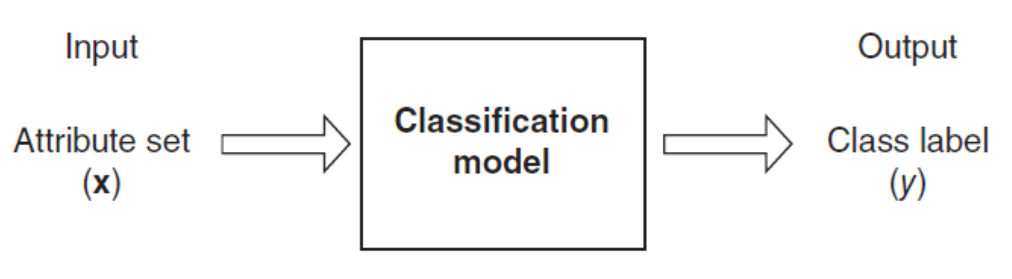
\includegraphics[scale = 0.6]{Images/classification.png}
    \caption{A schematic illustration of a classification task by Tan et al. \cite[p.~134]{DBLP:books/aw/TanSKK2019}.}
    \label{fig:classifiation}
\end{figure}


%\TODO{maybe difference opinion, sentiment, subjectivity?}
%According to Pang and Lee sentiment analysis "deals with the computational treatment of [...] opinion, sentiment, and subjectivity in text" \cite[p.~5]{DBLP:journals/ftir/PangL07}.  Pang and Lee suggest several applications for sentiment analysis, such as review-related websites, in addition to existing technologies such as recommendation systems, as well as business and government intelligence \cite[p.~8]{DBLP:journals/ftir/PangL07}.

\section{Sentiment Analysis}


\subsection{Definition}


Liu defines sentiment analysis, also known as opinion mining, as "the field of study that analyzes people's opinions, sentiments, appraisals, attitudes, and emotions toward entities and their attributes expressed in written text" \cite[p.~1]{liu_2015}. He states that entities include "products, services, organizations, individuals, events, issues, or topics" \cite[p.~1]{liu_2015}. He further analyzes the difference between sentiment and opinion, citing the Merriam-Webster dictionary. There, "sentiment is defined as an attitude, thought, or judgment prompted by feeling, while opinion is defined as a view, judgment, or appraisal formed in the mind" \cite[p.~2]{liu_2015}. Considering this definition, a subtle difference can be seen, where sentiment tends to be viewed more as a feeling, while an opinion is a more concrete view. Although this difference exists, sentiment analysis and opinion mining are still used interchangeably to refer to the same field. Liu defines the term opinion as an encompassing term that includes not only sentiment, but also additional information, such as the opinion holder. A more formal definition of an opinion by Liu can be seen in Equation \eqref{eq:opinion}.
\begin{equation}
    opinion = (e, a, s, h, t),
    \label{eq:opinion}
\end{equation}
where $e$ denotes an entity, $a$ is the target aspect of $e$, $s$ represents the sentiment, $h$ describes the opinion holder, and $t$ the time when the opinion was published \cite{liu_2015}. To further illustrate the difference, the example sentence "I like the display of my Dell laptop", published on 07.05.2022 by Max Mustermann is considered. Here, the entity $e$ is the target of the opinion, the Dell laptop, while $a$ is the specific attribute of the laptop that the sentiment relates to, the display. The sentiment $s$ is qualified as positive, the opinion holder $h$ is Max Mustermann, and the time $t$ is 07.05.2022, resulting in the quintuple (Dell laptop, Display, Positive, Max Mustermann, 07.05.2022). If an opinion does not target a specific aspect, but rather the entire entity, the aspect is defined as "GENERAL" \cite{liu_2015}. 


Liu identifies three different levels of analysis. The document level classifies an entire document as positive or negative, while assuming that it relates to a single entity, such as a product review. The next level is the sentence level, which determines the sentiment of each sentence, including neutral if it does not contain an opinion. The aspect level includes the entity and aspect with which an opinion is concerned \cite{liu_2015}.

Most research differentiates between two tasks in sentiment analysis. Pang and Lee, for example, differentiate between detection of polarity and detection of subjectivity. The most common form of polarity detection is called sentiment polarity classification, which aims to label an opinionated document as either positive or negative. Polarity may also be viewed as a multiclass problem, where the degrees of positivity are considered, as well as the neutral class, which Pang and Lee describe as the middle ground between positive and negative. Subjectivity detection, on the other hand, seeks to determine whether a given text contains a subjective opinion or is objective. Pang and Lee note that they make a distinction between neutral and objective, the latter being a lack of opinion \cite{DBLP:journals/ftir/PangL07}. Other researchers such as Liu define neutral as being the lack of opinion, noting that an objective sentence may still imply sentiment \cite{liu_2015}. Especially in human-coded data sets, the difference between objective and neutral is often problematic. For example, Nakov et al. instructed their coders to determine whether a sentence is objective, positive, negative, or neutral. Once Nakov et al. used this data set in their sentence polarity task, they combined sentences with an objective and neutral score to one class, as the coders often confused the two classes \cite{nakov-etal-2013-semeval}.

\begin{figure}
    \centering
    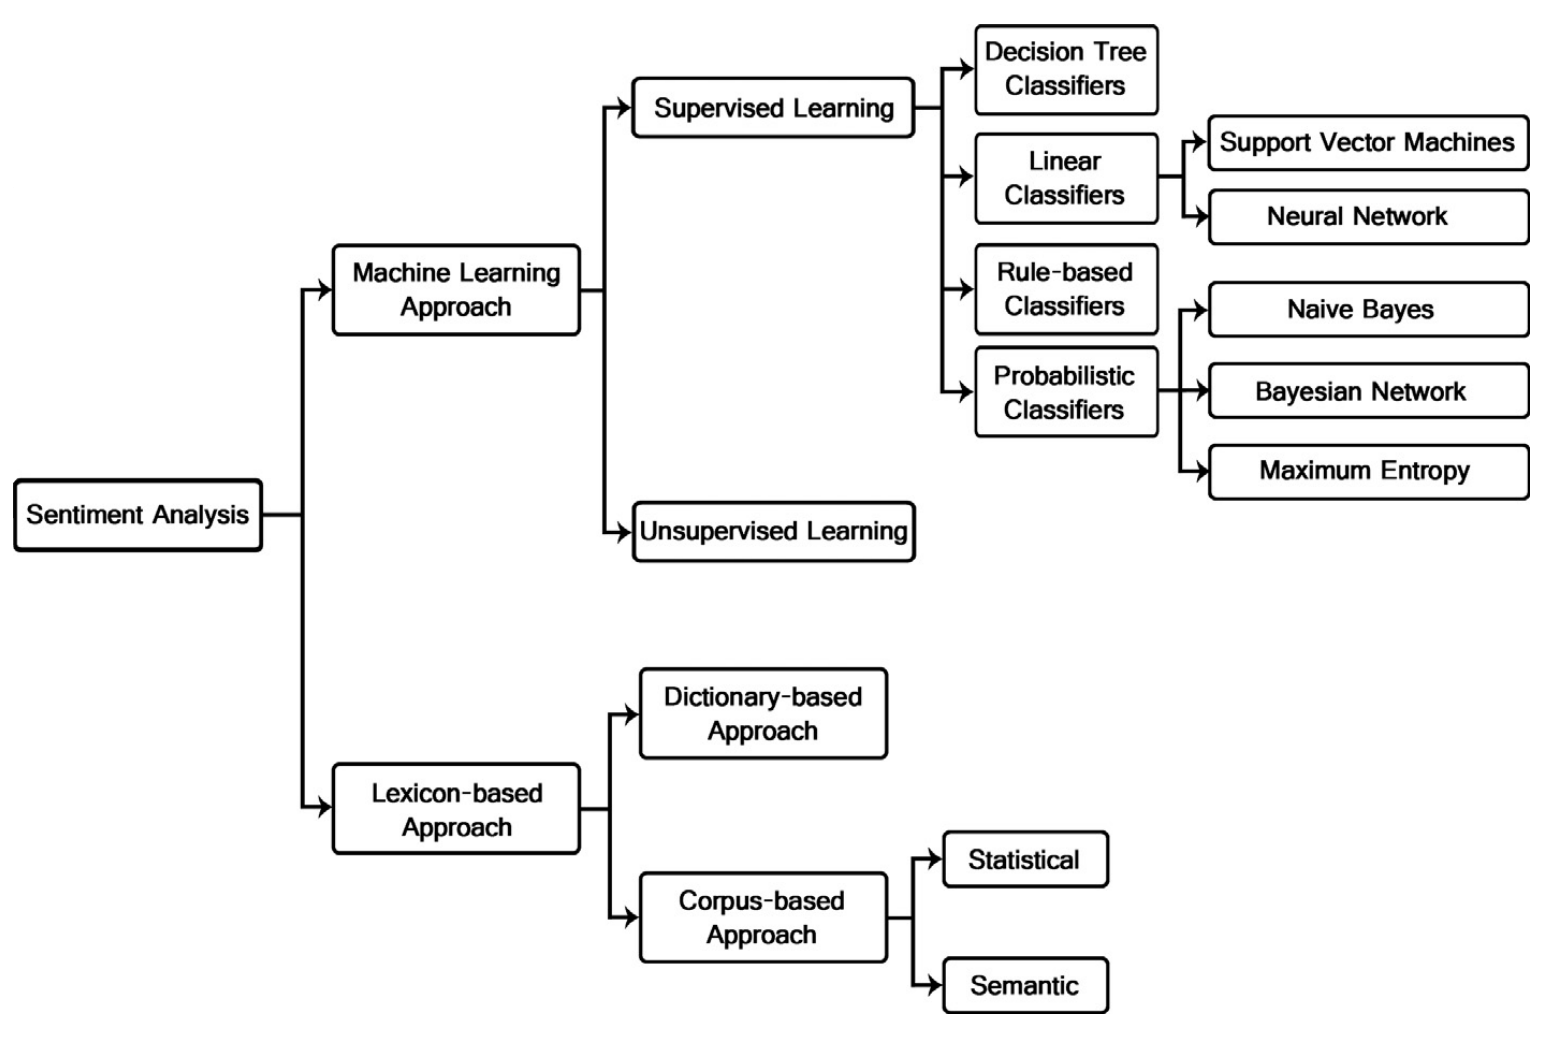
\includegraphics[scale=0.3]{Images/classification_techniques.png}
    \caption{Sentiment classification techniques by Medhat et al. \cite{MEDHAT20141093}.}
    \label{fig:classifiers}
\end{figure}

\subsection{Approaches}
For polarity classification, Medhat et al. divide techniques into three categories, machine learning, lexicon-based, and hybrid \cite{MEDHAT20141093}. Giachanou and Crestani identify a fourth technique, graph-based methods, \cite{DBLP:journals/csur/GiachanouC16}, which are not considered in this thesis. The most important classifiers are shown in Figure \ref{fig:classifiers}. 

\subsubsection{Machine learning classifiers}
\label{sub:fund_mach}
In general, the machine learning approach treats sentiment analysis as a text classification problem, employing training data to classify unknown instances. Supervised machine learning utilizes labeled training documents together with classifiers such as Naive Bayes. Because it can be difficult to generate a large number of labeled training data, unsupervised approaches are also applied, which rely solely on unlabeled data \cite{MEDHAT20141093}. The supervised methods are further subdivided. According to Tan et al., probabilistic classifiers, such as Naive Bayes and Logistic Regression, "make use of probability theory to represent the relationship between attributes and class labels" \cite[p.~414]{DBLP:books/aw/TanSKK2019}. Linear classifiers, on the other hand, try to find a hyperplane to separate instances from different classes \cite{MEDHAT20141093}. Decision Tree Classifiers, such as Random Forest, use attribute values to divide data into a tree structure. Finally, rule-based classifiers utilize a set of rules to classify an instance \cite{DBLP:books/aw/TanSKK2019}.

Feature selection is one of the essential parts of machine learning, as a classifier relies on the provided attributes. Giachanou and Crestani identify several different possible features for Twitter sentiment analysis: (1) Semantic features, for example, sentiment words and negations, which are extracted using lexicons; (2) Syntactic features, such as the presence of a word or term; (3) Stylistic features, which include emoticons and punctuation; and (4) Twitter-specific features, for example, hashtags or the number of replies \cite{DBLP:journals/csur/GiachanouC16}. For syntactic features, approaches differentiate on how to implement them. Some approaches look at each word of a tweet separately, which is called the unigram model, while others combine two (bigram model) or more words (n-gram model) as a combined feature.

\subsubsection{Lexicon-based methods}
\label{sub:fund_lex}
As stated previously, the lexicon-based approach needs a sentiment lexicon to identify sentiment words and their polarities. In addition, modifiers such as intensifiers and negations can be included to adjust sentiment values \cite{liu_2015}. There are three different methods for building a sentiment lexicon, which are outlined by Medhat et al. There is the manual collection of words, which is very time-intensive. A dictionary-based approach, which starts with a small list of sentiment words, can also be used. It subsequently searches dictionaries for synonyms and antonyms of the sentiment words, maintaining the orientations for synonyms and reversing them for antonyms. The found words are then added to the list and considered in the next iteration. The corpus-based approach utilizes context-specific orientations along with a list of opinion words to find other opinion words in a large corpus. It is based on sentiment consistency, which assumes that adjectives conjoined by "and" have the same polarity, while "but" would signify opposing polarities. This approach can be further subdivided into statistical approaches, which find words using statistics, and semantic approaches, which utilize semantic relationships \cite{MEDHAT20141093}.

\subsubsection{Hybrid methods}

Hybrid methods combine lexicon-based and machine learning methods to balance their disadvantages. Lexicon-based methods are inherently static, as they depend on a set list of words. If a tweet contains words that do not appear in the lexicon, the lexicon-based method can not classify it. On the other hand, a machine-learning method requires a large amount of labeled training data that is not easy to obtain manually. Approaches include using the lexicon-based score as an additional feature for the machine learning classifier, or employing multiple different classifiers by, for example, voting on the result \cite{DBLP:journals/csur/GiachanouC16}.


\section{Twitter}
Twitter is a microblogging service, which allows users to send messages, so-called "tweets", containing text, media, and URLs \cite{DBLP:journals/csur/GiachanouC16}. It is one of the largest social media platforms with 330 million monthly users in the first quarter of 2019, who posted 500 million messages daily \cite{twitter:users}. According to Pew Research Center, 23\% of U.S adults used Twitter, and the platform also had the second lowest age gap among the most popular social media platforms \cite{pew:socialmedia}. The length of a tweet was originally restricted to 140 characters until the company expanded the size to 280 characters in 2017 \cite{twitter:characters}. Due to this, Twitter offers a large number of short messages on varying topics made by varying user groups. 

Figure \ref{fig:example_tweet} shows an example of a tweet made by NASA for the Phoenix mission. An account is identified by its unique username, in the example tweet "@MarsPhoenix". There are several ways to interact with a tweet. A tweet can be (1) replied to, (2) retweeted, which shares the tweet to a user's profile, (3) quoted, which adds a comment to the retweet, or (4) liked. Other users can also be mentioned in a tweet, with their username being identified by the "@" character. 

\begin{figure}
    \centering
    
\includegraphics[scale=0.3]{Images/twitter_image.png}
    \caption{Picture of a tweet made by the @MarsPhoenix account \cite{twitter:tweet}.}
    \label{fig:example_tweet}
\end{figure}

Twitter's characteristics lead to challenges when applied to sentiment analysis, which are outlined by Giachanou and Crestani. The short length of tweets differs from other domains often used in sentiment analysis, such as movie reviews, which are much longer. Bermingham and Smeaton concluded that classification of sentiment on microblogs is easier than classifying longer documents \cite{microblogs}.

The informal nature of Twitter and its length restrictions frequently lead to abbreviations, slang, and misspellings, which must be considered. Especially emphatic lengthening, which refers to the usage of repeated letters in order to amplify a word, for example, "gooood", is very common in Twitter \cite{DBLP:journals/csur/GiachanouC16}. These characteristics lead to data sparsity, since many terms appear infrequently over an entire corpus of tweets \cite{DBLP:journals/csur/GiachanouC16}. Tan et al. define that for sparse data, most attribute values of a data object are 0 \cite{DBLP:books/aw/TanSKK2019}. Applied to sentiment analysis, the vast majority of observed words, and thus features, do not appear in a tweet. Saif et al. observed that 93\% of the words in their Twitter corpus occurred less than 10 times, compared to 78\% in movie review data \cite{data_sparsity}. 

Twitter offers two APIs to retrieve and analyze Twitter data, REST and streaming \cite{DBLP:journals/csur/GiachanouC16}. There currently are three different access levels, which provide different rates and limits. The elevated level, for example, allows the retrieval of up to 2 million tweets per month \cite{twitter:about}. The REST API provides a short-lived connection, through which several functionalities can be accessed, such as the lookup, creation, and deletion of tweets. Most importantly, it can also be used to search for tweets. Twitter differentiates between recent search, which provides access to public tweets posted in the last week, and full-archive search, which enables access to every tweet ever made. For full-archive search, academic research access is needed. Tweets can be filtered according to parameters such as language, content, and type (e.g. retweet) \cite{twitter:search}. 

On the other hand, the streaming API allows developers to access a real-time stream of tweets, which can be filtered using rules \cite{twitter:stream}. All information is returned in a JSON format, which can be easily parsed by many programming languages. Thus, the Twitter API provides a great method to collect large amounts of tweets \cite{DBLP:journals/csur/GiachanouC16}.





\chapter{Methodology and Implementation}
\label{cha:Chapter4_Methodology}

Length: 20-25 pages

Effort: 8 weeks+

Teilung zwischen Methodik (eher abstrakt) und Implementierung
Damit beginnen --> also mit Implementierung

Questions:
\begin{itemize}
\item Structure --> differentiation between getting the data, analysing the data and evaluating the results ok? --> Kann man machen
\item General idea: ``Readers should be able to carry out the same procedure using the thesis'' --> level of detail, e.g. cloud services? --> Implementierung auch auf Github zur Verfügung stellen, API auf höherem Level (was machen die Funktionen verwenden),
Falls Cloud: nur virtueller Rechner --> eher nicht wichtig, falls spezifische Dienstleistung z.B. OpenAI (KI, Parsing) --> dann detaillierter, eher Richtung Implementation
\item Case study --> Evaluation of accuracy based on one real life topic? Topic, e.g. Covid-19 pandemic, german elections (aufpasssen, Politik schwer!), ...? --> je nach Umfang auch mehrere (sollen sich unterscheiden, Covid sehr viele Bereiche), Tweets auch auf Englisch
\end{itemize}

Content
\begin{itemize}
\item Data 
\begin{itemize}
    \item What data does twitter provide, auch z.B. Likes, Retweets
    \item Data extraction, Cloud Services --> spezifischer Dienst?
\end{itemize}
\item Analysis
\begin{itemize}
    \item Lexicon-Based Method
    \item Machine Learning Based Method
    \item Hybrid Method
\end{itemize}
\item Evaluation
\begin{itemize}
    \item Parameters --> objektive Kriterien, Qualität der Analyse Methode + Begründung der Kriterien, Komplexität (Laufzeitkomplexität ja, Implementierung --> an sich nicht schlimm, aber robust? Abstürze?)
    \item Case Study
    \item Qualität der Ergebnisse --> gut/schlecht, kann das akkurat erkannt werden?, evtl. menschliche Analyse, schöner: auf subjektive Einschätzung verzichten
\end{itemize}
\end{itemize}




\chapter{Conclusion}
\label{cha:Chapter5_Conclusion}

Length: 1-2 pages

Effort: 1-2 days


Zusammenfassung der Ergebnisse, Ausblick --> was kann man noch machen, auf Ergebnisse aufbauen, weiterführende Themen

Beim Erstellen der Arbeit --> nicht jeder Idee hinterherrennen, eher dann für Conclusion

Implementation source code --> muss nicht sein, kann auch ein link auf github sein



% Literaturverzeichnis
\newcommand{\Literatur}{Bilbiography}
\addcontentsline{toc}{chapter}{\Literatur}
\nocite{*}
\bibliography{Literaturverzeichnis/literatur}


% Fügt Anhang zum Dokument hinzu
\appendix
\chapter{Implementation source code}
%\addcontentsline{toc}{chapter}{Appendix}
%\include{Appendix/Appendix}
%\include{Appendix/Code}


\end{document}
